% https://tex.stackexchange.com/a/280454
\documentclass[tikz,varwidth,border=7mm]{standalone}
\usetikzlibrary{math}
\begin{document}
  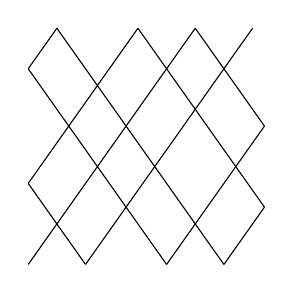
\begin{tikzpicture}[scale=3]
      \tikzmath{
        % initial value, max value, next bounce value, speed
        \x = 0; \maxx=1; \bx=\maxx; \dx = 1;
        \y = 0; \maxy=1; \by=\maxy; \dy = 1.41421356237;
        for \i in {0,...,10}{
          % save values
          \sx = \x; \sy = \y;
          % time to next bounce
          \tx = (\bx-\x)/\dx;
          \ty = (\by-\y)/\dy;
          if \tx < \ty then { % if bounce on x before y
            \x = \bx;
            \bx = \maxx-\x;
            \dx = -\dx;
            \y = \y + \tx*\dy;
          } else { % if bounce on y before x
            \y = \by;
            \by = \maxy-\y;
            \dy = -\dy;
            \x = \x + \ty*\dx;
          };
          {\draw (\sx,\sy) -- (\x,\y);};
        }; % end for
      };
  \end{tikzpicture}
\end{document}
